\documentclass[10pt,a4paper, twocolumn]{article}
%\documentclass[10pt,a4paper]{article}
\usepackage[latin1]{inputenc}
\usepackage{graphicx,epsfig}
\usepackage[reqno,centertags]{amsmath}
\usepackage{amsmath}
\usepackage[top=2cm, bottom=2cm, left=2cm, right=2cm]{geometry}
\usepackage{enumitem}					% For the margin in "itemize"
\usepackage{indentfirst}				% To indent first paragraph
\usepackage{tabularx}					% To have tables of full width
\usepackage[lofdepth,lotdepth]{subfig}	% For subfigures
\usepackage[hidelinks]{hyperref}		% For links in PDF
\usepackage{textcomp}					% For ~
\usepackage{amsfonts}					% For sets
\usepackage{amssymb}					% For maths
\usepackage[lofdepth,lotdepth]{subfig}	% For subfigures
\usepackage{float}						% For floating images
\usepackage{sectsty}					% To configure sections fonts
\usepackage[boxed, linesnumbered]{algorithm2e}	% For algorithms
\usepackage{multirow}					% For multirows in tables


% Title declaration
\title{\LARGE \bf
UKF Localisation of a Formula Student Car
}
\author{Corentin Chauvin-Hameau}
\date{January 2019}

% Abstract configuration
\renewenvironment{abstract}{\bf \textit{Abstract} ---}


\begin{document}

% Configuration
\renewcommand{\thesection}{\Roman{section}.}		% change numerotation style
\renewcommand{\thesubsection}{\Alph{subsection}.}	% ...
\sectionfont{\normalfont}				% change section formating
\subsectionfont{\normalfont\itshape}	% change subsection formating
\setlist[itemize]{noitemsep, itemsep=2pt}
\setcounter{secnumdepth}{2}  % remove numerotation for subsubsection and above
%\setlength{\columnsep}{0.5cm}	% change the space between the columns


% TITLE and ABSTRACT
\maketitle

\begin{abstract}
This report presents the implementation of an Unscented Kalman Filter used for the localisation of a driverless racing car taking part in Formula Student competitions. The UKF can fuse the data measured by the various sensors mounted on the car (IMU, odometry, GNSS and cones perception). The development is done under the Robot Operating System and using a custom Gazebo simulation providing realistic data.
\end{abstract}


% SECTION: Introduction
\section{INTRODUCTION}

\subsection{Problem description}
\begin{figure}[h]
	\centering
	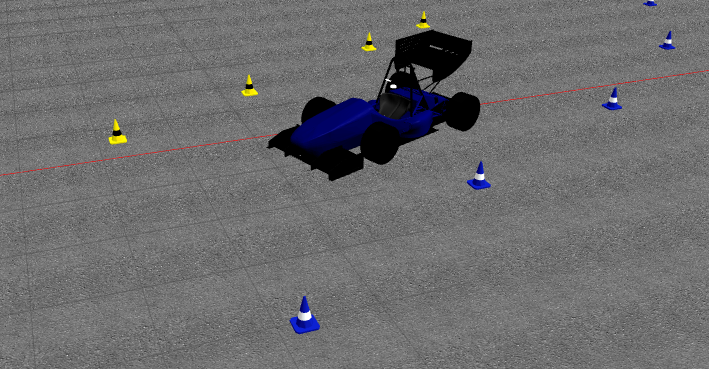
\includegraphics[width=\columnwidth]{images/gazebo_simulation.png}
	\caption{Gazebo simulation}
	\label{fig:gazebo_simulation}
\end{figure}
	
Formula Student is an engineering competition where student teams from all over the world design and build formula racing cars. Since a few years it presents a driverless category, which requires the car to complete several laps autonomously. Here, determining the position of the car is a core issue, and is helped by several sensors embedded in the car. The Formula Student car of KTH (the one which is considered for this project) is equipped with:
\begin{itemize}
	\item an Inertial Measurement Unit (IMU) measuring linear accelerations and orientation velocities
	\item wheel encoders providing odometry
	\item a standard GNSS giving position and velocity. Actually, the IMU and the GNSS measurements are provided by the same sensor, and the data can already be fused by its internal algorithms. However, the measurements will be handled as if it was given by separate sensors.
	\item cones position detection. The track is delimited by cones on its sides (see figure \ref{fig:gazebo_simulation}). During the competition, the position of the cones is not known at the beginning. However, the mapping and the data association won't be considered in this report, so the absolute position of the cones will be assumed to be known.
\end{itemize}

The car and its sensors are simulated in Gazebo. The car motion and dynamics are faithful to the real car. The IMU and the GNSS are simulated by plugins reproducing typical behaviours of these sensors, with noise parameters calibrated to fit the actual sensors mounted on the car. The odometry is generated taking the ground truth given by Gazebo, and adding noise, mainly according to the \textit{odometry motion model} in \cite{ProbabilisticRobotics} (section 5.4) (it won't be presented in this report). The real car can either detect the cones thanks to a stereo camera, or a lidar. The cones detection will be faked by adding a Gaussian noise of constant variance to the cones position given by Gazebo. 

All the simulated output are in the same format and naming as for the real car. Therefore, the developed algorithm can be used on the real car without modification.\\

The main goal of the project is to fuse the different measurements with an Unscented Kalman Filter, to estimate the pose and the twist of the car. The structure of the algorithm is mainly based on \cite{RobustVehicleLocalization} which describes a UKF for an autonomous car equipped with an IMU, a DMI (Distance Measuring Instrument) and a GNSS. The application and the sensors are very similar, so it seems to be a very good starting point.

Some additions have to be made to handle the extra data measured by the sensors that we have. For instance, DMI is providing information about the linear speed of the car, while wheels odometry gives information about the linear and angular speeds of the car. Moreover, the GNSS speed is not fused in the article, while the speed is often much more accurate than the position with this kind of sensors. Indeed, the speed can be determined accurately by using Doppler effect on the motion of the satellites, as explained in \cite{ GNSSVelocity}. Finally, the cones detection can give information about the absolute position of the car, with relatively high accuracy (the lidar is for instance detecting cones with an accuracy of 3 cm).


\subsection{Contribution}
The contribution of this project is about:
\begin{itemize}
	\item providing a full Gazebo simulation of the car and its sensors
	\item implementing the UKF of \cite{RobustVehicleLocalization} and adapting it
	\item developing the measurement models for the odometry, the GNSS speed and the cones
\end{itemize}

The Gazebo simulation is highly based on the code of the Formula Student team of Edinburgh (sources on GitHub: \url{https://github.com/eufsa/eufs_sim}). What remained was to adapt the sensors used by the KTH Formula Student team, fake the cones detection and noise the odometry. I was asked to develop this simulation for the KTH team, so my work will not only be used for this project.

In the UKF algorithm, the prediction phase of \cite{RobustVehicleLocalization} was to be adapted, since the state is slightly different here (see next section).


% SECTION: UKF localisation
\section{UKF LOCALISATION}

\subsection{Algorithm}

\begin{algorithm}[h]
	\SetAlgoNoLine
	\DontPrintSemicolon
	\SetNlSkip{12pt}
	
	\SetKwProg{UKF}{UKF\_localisation(}{ ):}{}
	
	\UKF{$\mu_{t-1}, \Sigma_{t-1}, u_t, z_t$}{
		\textit{// Prediction}\;
			$\chi_{t-1} = [\mu_{t-1}, \mu_{t-1} \pm (\sqrt{(n+\kappa)\Sigma_{t-1}})_i]$\;
			$\bar\chi_t = predict(\chi_{t-1}, u_t) $\;
			$\mu_t = \sum_{i=0}^{2n} w_m^{(i)} \bar\chi_t^{(i)} $\;
			$\Sigma_t = \sum_{i=0}^{2n} w_c^{(i)} (\bar\chi_t^{(i)}-\mu_t)(\bar\chi_t^{(i)}-\mu_t)^T + Q$\;
		\;
		\textit{// Measurement update}\;
		\ForEach{sensor measurement available $z_t$}{
			$\bar \chi_t = [\mu_{t-1}, \mu_{t-1} \pm (\sqrt{(n+\kappa)\Sigma_{t-1}})_i]$\;
			$Z_t = measurement\_model(\bar \chi_t, z_t)$\;
			$\hat z_t = \sum_{i=0}^{2n} w_m^{(i)} Z_t^{(i)}$\;
			$S_t = \sum_{i=0}^{2n} w_c^{(i)} (Z_t^{(i)}-\hat z_t)(\bar z_t^{(i)}-\hat z_t)^T + R $\;
			$\Sigma_t^z = \sum_{i=0}^{2n} w_c^{(i)} (\bar \chi_t^{(i)}-\mu_t)(Z_t^{(i)}-\hat z_t)^T$\;
			$K_t = \bar\Sigma_t S_t^{-1}$ \;
			\;
			$\mu_t = \mu_t + K_t (z_t-\hat z_t)$\;
			$\Sigma_t = \Sigma_t - K_t S_t K_t^T$\;
		
		}
		\;
		\Return{$\mu_t, \Sigma_t$}
	}
	\caption{Unscented Kalman Filter}
	\label{algo:UKF}
\end{algorithm}

This section describes the implemented algorithm. Its structure is the same as the classical one in \cite{ProbabilisticRobotics}, and the prediction is almost as in \cite{RobustVehicleLocalization}. The state that we will try to estimate is $(x, y, \theta, v_x, v_y,  \omega)$, where $(x, y)$ is the absolute position of the car, $\theta$ is its heading, $v_x$ is its longitudinal speed, $v_y$ is its lateral speed, and $\omega$ is its angular speed.

As said previously, the state is slightly different from the one in \cite{RobustVehicleLocalization}. Indeed, we will assume that the car is on a plane and work in 2D. Moreover, $\omega$ is added in the state since the UKF will fuse the angular speed from the odometry.

In the paper, the lateral speed is estimated in the prediction phase with the lateral acceleration given by the IMU, and never updated in the update phase. This is problematic because the IMU has always small biases, and it will accumulate errors through time. In our case, GNSS twist measurements will give additional information about the lateral speed, and will prevent these effects. However, when the GNSS twist is not fused, the lateral speed will be assumed to be zero.\\

At each time instant $t$, the UKF algorithm can be split into two different phases: a \textit{prediction} phase where the filter tries to estimate the relative motion of the car, and an \textit{update} phase where it takes into account sensors readings to correct the state.

\subsubsection{Prediction phase}
In the prediction phase, 13 \textit{sigma points} are generated around the state estimate $\mu_{t-1}$ (see line 3 in algorithm \ref{algo:UKF}), two by dimensions (here $n=6$) and the state estimate itself. The way the sigma points are initially spread depends on the state covariance $\Sigma_{t-1}$. If the uncertainty on the state is big, the points will be spread a lot. The motion of each sigma points is estimated by the prediction function, and a new state can be computed by averaging these sigma points (lines 4 and 5). The average is weighted so that the sigma point corresponding to $\mu_{t-1}$ is given more weight than the others. Likewise, a new state covariance $\Sigma_t$ is computed by averaging the covariance of each sigma points (line 6). A way to compute $w_c$, $w_m$ and $\kappa$ can be found in \cite{UKFForNonLinearEstimation}.

\begin{algorithm}[h]
	\SetAlgoNoLine
	\DontPrintSemicolon
	\SetNlSkip{-1.01\columnwidth}
	
	\SetKwProg{predict}{predict(}{ ):}{}	
	\predict{$\chi_{t-1}, u_t $}{
		\ForEach{sigma point $(x_t^i, y_t^i, \theta_t^i, v_{x, t}^i, v_{y, t}^i, \omega_t^i)$}{
			$x_{t+1}^i = x_{t}^i + (v_{x, t}^i \cos(\theta_t^i) - v_{y, t}^i \sin(\theta_t^i)) \delta_t$ \;
			$y_{t+1}^i = y_{t}^i + (v_{x, t}^i \sin(\theta_t^i) + v_{y, t}^i \cos(\theta_t^i)) \delta_t$ \;
			$\theta_{t+1}^i = \theta_t^i + \omega_t^i \delta_t$ \;
			$v_{x, t+1}^i = v_{x, t}^i + u_t[a_x] \delta_t$ \;
			$v_{y, t+1}^i = v_{x, t}^i + u_t[a_y] \delta_t$ \;
			$\omega_t^i = \nu \omega_t^i + (1-\nu) u_t[\omega]$ \;
		}
		\;
		\Return{$\bar\chi_t$}
	}
	
	\caption{Prediction phase}
	\label{algo:predict}
\end{algorithm}


%For that, the following parameters are needed:
%$$ \begin{array}{l c l}				
%	\kappa 	&=& \alpha^2 (n + \gamma) - n \\
%	w_m^0 &=& \kappa / (n + \kappa) \\
%	w_c^0 &=& \kappa / (n + \kappa) + 1 - \alpha^2 + \beta \\
%	w_m^i &=& w_c^i \ \ = \ \ 1 / ((2(n+\kappa)) \text{\ \ \  for }i=1...2n
%\end{array} $$
%We can find values for the different constants with to \cite{UKFForNonLinearEstimation}. 


The algorithm presented by \cite{RobustVehicleLocalization} uses the data from the IMU for the prediction of the linear speeds. With the same idea, we will use the IMU angular speed $u_t[\omega]$ to also update $\omega$ (line 8 of algorithm \ref{algo:predict}). This weird thing with the $\nu$ factor is a way to incorporate the angular speed fused from the odometry. If $\nu$ is small, a big weight is given to the IMU, while if $\nu$ is near 1.0, more weight is given to the odometry.

In a different spirit, a better idea could have been to fuse the IMU data in the update phase, and not in the prediction. For example, \cite{GeneralizedEKFImplementation} presents the implementation of the Extended Kalman Filter of a very common ROS package for localisation, \texttt{robot\_localization} (which also has a UKF). In this implementation, the state is also the full 3D pose and twist. The prediction is done by propagating the dynamical model, and the sensors readings are handled only in the update phase. This has the advantage of taking into account the covariance of the IMU and avoiding this $\nu$ trick.

\subsubsection{Update phase}
During the update phase, each sensor data is processed sequentially. Again, sigma points are generated with the same method as previously. A measurement model is used to predict the observation which could be done for each sigma point (more on the different measurement models used in the next subsection). An average $\hat z_t$ of these 13 observations is then computed (line 12 of algorithm \ref{algo:UKF}). Its uncertainty $S_t$ is computed using the measurement uncertainty matrix $R$, which depends on the sensor type (line 13). $\Sigma_t^z$ is the cross-covariance between the sigma points and the observation, and is used to compute the Kalman gain $K_t$ (line 15). The state is then corrected by comparing $\hat z_t$ to the actual measurement $z_t$, and its covariance decreased.


\subsection{Measurement models}
In the implementation, the different \textit{measurement\_model} functions return the predicted measurement $Z_t$ of all the sigma points, but also the true measurement $z_t$ itself and its uncertainty $R$. Since the lines 12 to 18 of algorithm \ref{algo:UKF} are handled by the same function for each sensor, the output of the \textit{measurement\_model} functions has to be of the same dimension.

The ROS measurement messages carry their own uncertainties, which has been tuned to be faithful to the data. This will be used for generating $R$. However, for some sensors (cones detection and GNSS position in particular), it was better not to use the uncertainties in the ROS messages, but rather have it as tunable parameters in order to adapt the influence of each measurement.

\subsubsection{Odometry model}
The odometry sensor is providing linear speed $v_x$ and angular speed $\omega$. The measurement vector is then $z_t = (0, 0, 0, v_x, 0, \omega)$. For each sigma point, the projected measurement is $Z_t^{(i)} = (0, 0, 0, v_{x, t}^{(i)}, 0, \omega_t^{(i)})$. Finally, the uncertainty matrix is $R = diag(a, a, a, \sigma_{v_x}^2, a, \sigma_\omega^2)$ where $a$ is a big number preventing the measurement on the pose to have to much influence (for example $10^{15}$).

\subsubsection{GNSS pose model}
This one is the same as in \cite{RobustVehicleLocalization}. A GNSS is able to estimate its latitude and longitude, and then a ROS package converts it in a Cartesian absolute frame (for example pointing to the East). This absolute frame has to be the same as the frame in which the state is estimated (or conversion has to be done). The true measurement is therefore $z_t = (x, y, 0, 0, 0, 0)$. For each sigma point, $Z_t^{(i)} = (x_t^{(i)}, y_t^{(i)}, 0, 0, 0, 0)$.

The uncertainty matrix is $R = diag(\sigma_x^2, \sigma_y^2, a, a, a, a)$ where the $\sigma$ are tunable parameters in this case. We will see it in the experimentations, the influence of this measurement is very important. For low values of $\sigma$, the estimated pose of the car is very shaky, as the measurement. For high values, the influence of the GNSS becomes negligible. A good balance has to be found.

\subsubsection{GNSS twist model}
The GNSS gives $(v_x^0, v_y^0)$ in the absolute frame, while the estimated speed of the car is aligned with its heading. To bring the measurement back in the good frame, we will use the track (the direction of the speed) $\varphi = \text{atan2}(v_y^0, v_x^0)$ which we will assume equal to the heading of the car. This assumption holds when the amount of slip is not too important. Therefore,
$$ \begin{array}{l c r}				
	v_x &=& v_x^0\cos(\varphi) + v_y^0\sin(\varphi) \\
	v_y &=& -v_x^0\sin(\varphi) + v_y^0\cos(\varphi)
\end{array} $$
We can also use this track to update the heading of the car. This is very valuable because it is the only sensor giving absolute information about the heading. The measurement vector is then $z_t = (0, 0, \varphi, v_x, v_y, 0)$. For each sigma point, $Z_t^{(i)} = (0, 0, \theta^{(i)}, v_{x, t}^{(i)}, v_{y, t}^{(i)}, 0)$.

The uncertainty on the speeds is contained in the ROS message, but not the uncertainty on the track. By differentiating the formula computing $\varphi$, we can compute $\sigma_\varphi^2 = ((v_x\sigma_{v_y})^2 + (v_y\sigma_{v_x})^2) / (v_x^2 + v_y^2)$. Then $R = diag(a, a, \sigma_\varphi^2, \sigma_{v_x}^2, \sigma_{v_y}^2, a)$. If the speed is small, the uncertainty on $\varphi$ is very big, and it is probably the same for the uncertainties on $v_x$ and $v_y$. Thus, the update is done only if the speed is above a specific threshold (1 m/s for example).

\subsubsection{Cones detection model}
The cones detection system is providing the noised position of each cones in range of detection in the sensor frame. The sensor is placed at the front of the car, on its $x$ axis. $(x_m, y_m)$ is then the position of the measured cone transformed into the car frame. We assume that we know the absolute position of the cones at the beginning and we don't care about data association. So for each detected cone, we have its absolute position $(x_b, y_b)$.

We will process each cone sequentially. If it is easier than taking into account all the cones at the same time, it presents two drawbacks:
\begin{itemize}
	\item for each cone update, the covariance of the state will decrease, which gives more weight to the first cones processed.
	\item an outlier could shift the state a lot, leading to bad data association when processing the next cones. This is not a problem in our assumptions.
\end{itemize}

A first idea could be to take $z_t = (x_b, y_b, 0, 0, 0, 0)$ as observation vector. For each sigma point, the predicted observation would then be the absolute position of the cone: $Z_t^{(i)} = (x^{(i)} + x_m\cos\theta^{(i)} - y_m\sin\theta^{(i)}, y^{(i)} + x_m\sin\theta^{(i)} + y_m\cos\theta^{(i)}, 0, 0, 0, 0) $. However, if the cone is a bit far, the measurement is very sensitive to $\theta^{(i)}$. This causes a problem in the update phase.

To see that, let's assume the state of the car is perfectly known, and that the cone measurement has no noise. $Z_t^{(i)}-z_t = 0$ for $i$ = 0 (the sigma point corresponding to the mean) and $i$ = 7 to 12. And $Z_t^{(i)} + Z_t^{(i+1)} - 2z_t = 0$ for $i$ = 1 and 3 (the sigma points where $x$ and $y$ is shifted by the same opposite constant). However, for the sigma points where the heading is shifted, we have $Z_t^{(4)} + Z_t^{(5)} - 2z_t \neq 0$. Therefore, $z_t - \hat z_t$ will be quite big, and the state will change a lot during the update. \\

A better idea is to take for each sigma point $Z_t^{(i)} = (x_t^{(i)}, y_t^{(i)}, 0, 0, 0, 0)$. The measurement is then the position of the car given the absolute position of the cone, the relative measurement and the estimated heading: $z_t = (x_b - x_m\cos(\theta) + y_m\sin(\theta), y_b - x_m\sin(\theta) - y_m\cos(\theta), 0, 0, 0, 0)$. This leads to much more stable behaviour. \\

An other problem was that the update was not only influencing the position, but also the heading with a big magnitude. A solution inspired by the \texttt{robot\_localization} package is to manually select the elements of the state which should be updated (in line 17 of algorithm \ref{algo:UKF}). Thus, only the position is updated, and the uncontrolled bad effects on the heading are removed. I however let the covariance update unchanged since the bad effects on the covariance were negligible.


% SECTION: SIMULATED RESULTS
\section{SIMULATED RESULTS}
In this section, the differences between the different sensors and their effect on the estimation are studied. The comparison will be done for one lap (about a hundred meters) where the car is driven manually, and with the Root Mean Square Errors (RMSE) in distance, linear speed, orientation and angular speed between the output of the UKF and the ground truth provided by the simulator: $RMSE_d = \sqrt{\sum_{t=1}^T [(x_0-x)^2 + (y_0-y)^2]/T}$ ($RMSE_v$ is computed the same way) and $RMSE_\theta = \sqrt{\sum_{t=1}^T (\theta_0-\theta)^2/T}$ ($RMSE_\omega$ is computed the same way).

For all the presented figures, the green curve corresponds to the ground truth, the blue curve corresponds to the output of the UKF, and the red curve corresponds to the noised odometry input. The scale of the grid is one meter per tile. The grey points are the undetected cones, and the colored points are the detected cones. In the tables, the values are given in International System of Units.

Often, at one point in the runs (in the bottom left corner of the pictures), the estimated orientation is doing something weird. The reason is not very clear, there is probably a mistake with a modulo somewhere in the code. Fortunately, it doesn't seem to affect the remaining of the runs.

\subsection{Dead reckoning}
Using only the prediction phase with the IMU leads to very poor results in position, even when the experiment is conducted with a noise free IMU. If the position is often very badly determined, the orientation is way better. This difference comes from different factors:
\begin{itemize}
	\item the position is obtained by integrating two times the linear acceleration given by the IMU, while the orientation is only the result of one integration of the angular speed.
	\item the simulated car is mounted on springs and dampers, which plays on its orientation during accelerations and decelerations. If the IMU is not perfectly horizontally oriented, gravity introduces additional biases. Taking into account the orientation of the IMU in the predict phase would be a good idea to deal with it.
\end{itemize}
It is hard to quantify the errors between the ground truth and the output of the filter because it varies a lot between each run. Figure \ref{fig:dead_reckoning} shows two typical runs, and table \ref{table:dead_reckoning} the corresponding offsets and RMSE.

\begin{figure}[h]
	\centering
	\subfloat[]{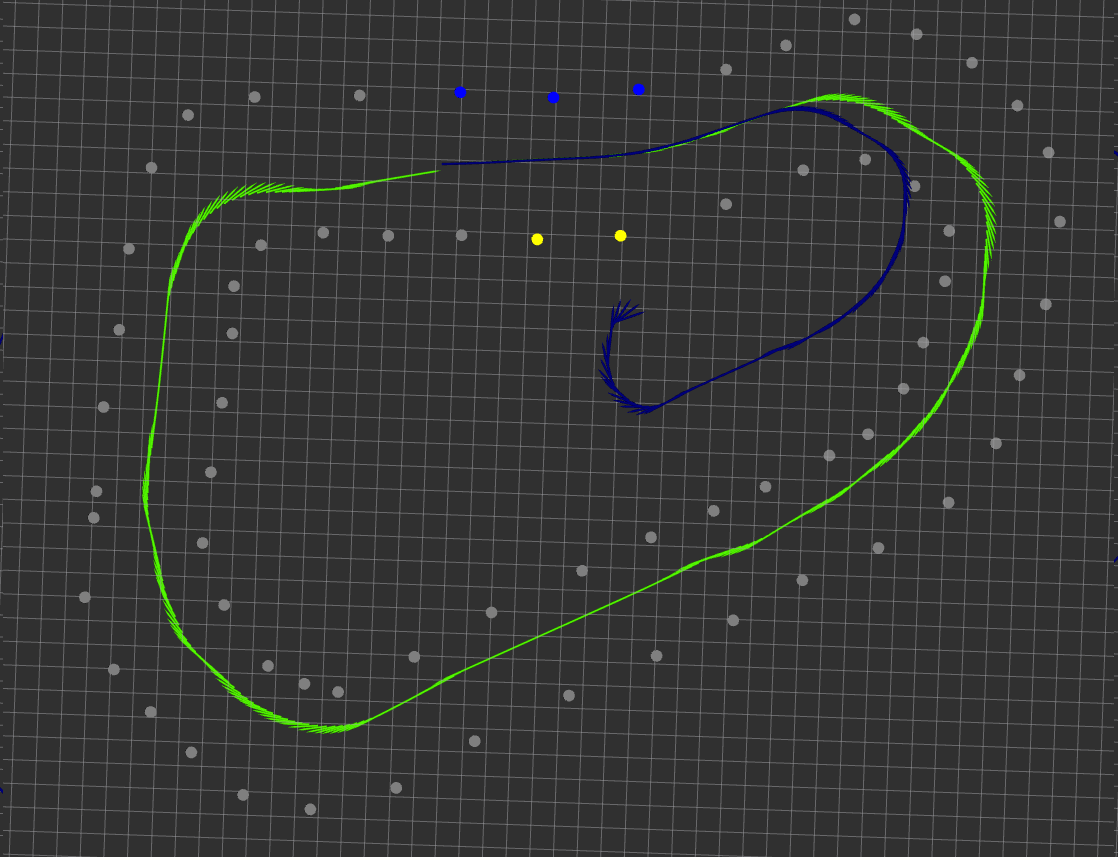
\includegraphics[width=\columnwidth]{images/dead_reckoning.png}}
	\newline
	\subfloat[]{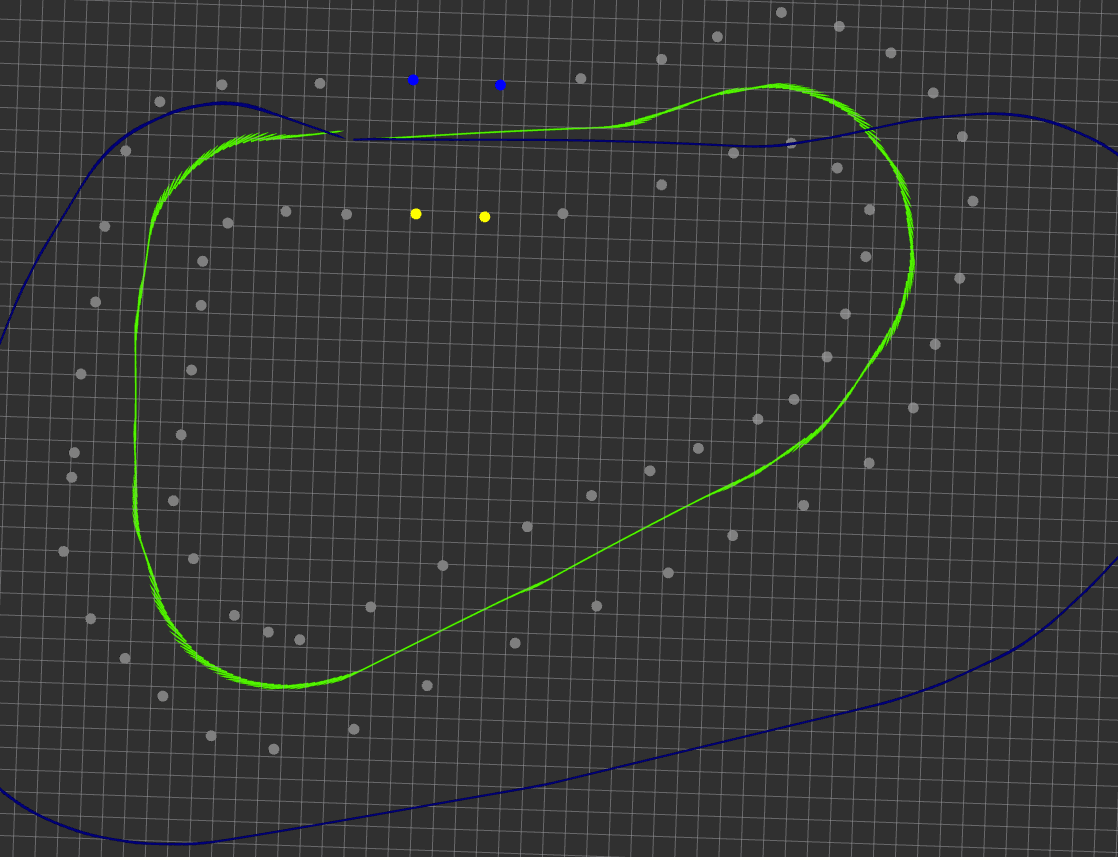
\includegraphics[width=\columnwidth]{images/dead_reckoning2.png}}	
	\caption{Dead reckoning (IMU only) for two different runs}
	\label{fig:dead_reckoning}
\end{figure}

\begin{table}[h]
	\begin{center}
		\begin{tabular}{|c|c|c|c|c|c|c|c|}
			\hline
			\multirow{2}{*}{\textbf{Run}} & \multicolumn{2}{c|}{\textbf{Final offsets}} &  \multicolumn{4}{c|}{\textbf{RMSE}} \\ \cline{2-7}
			  & $d$ & $\theta$ & $d$ & $\theta$ & $v$ & $\omega$ \\ \hline
			1 & 11.41 & 0.01 & 12.96 & 0.01 & 1.78 & 0.02 \\
			2 & 0.31 & 0.46 & 9.17 & 0.91 & 7.94 & 0.04 \\
			\hline
			
		\end{tabular}
		\caption{Final offsets and RMSE for dead reckoning}
		\label{table:dead_reckoning}
	\end{center}	
\end{table}

It becomes clear here that using the IMU in the prediction step was not necessarily a good idea. Using the linear speed provided by the odometry instead of the acceleration of the IMU could be better.

\subsection{IMU + odometry}
Fusing the odometry in the update phase helps to reduce the errors, but is not enough to reach an acceptable level. The differences between runs with same parameters are less important, so the results are easier to trust.

A big $\nu$ gives more weight to the angular speed of the odometry, and leads to slightly better results. However, even artificially decreasing the covariance of the odometry is not enough to get the output of the UKF looks like the odometry input.

\begin{figure}[h]
	\centering
	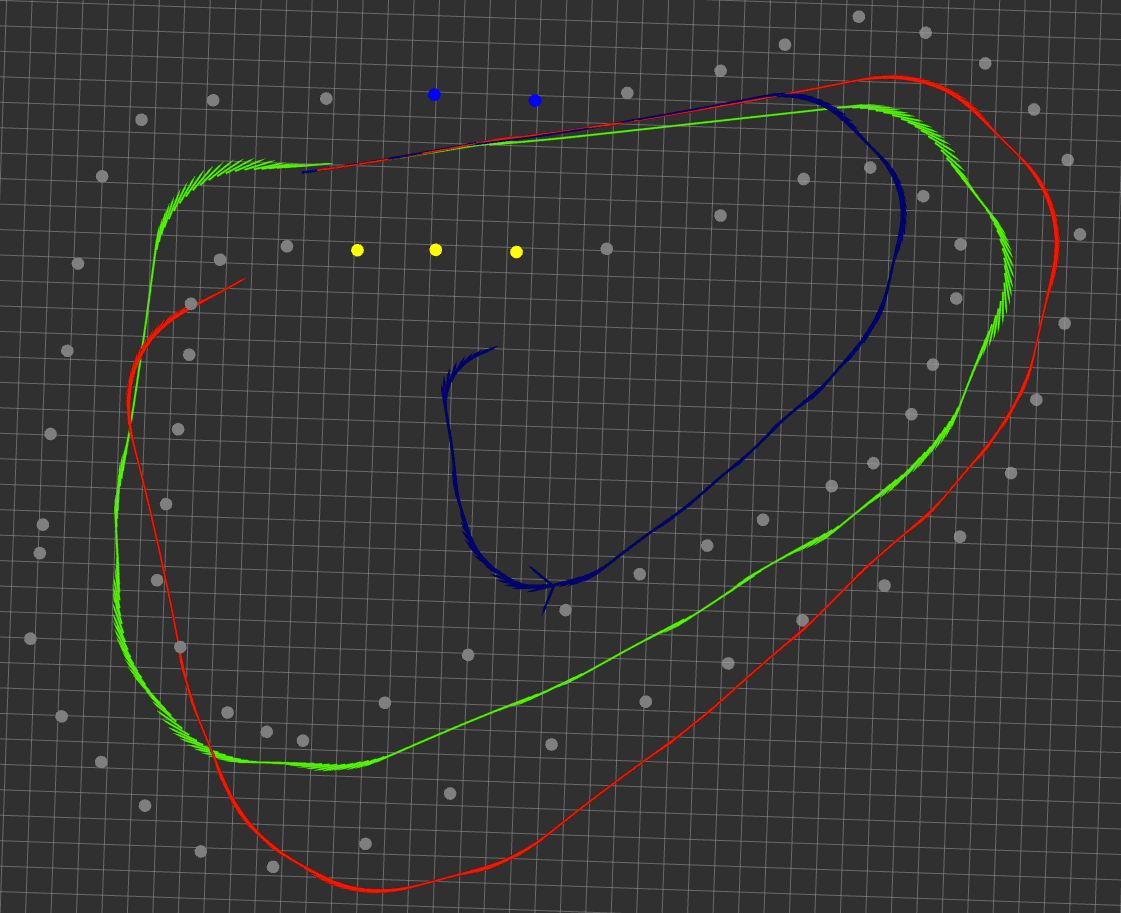
\includegraphics[width=\columnwidth]{images/odom2.png}
	\caption{Fusing IMU and odometry with $\nu=0.8$}
	\label{fig:odom}
\end{figure}

\begin{table}[h]
	\begin{center}
		\begin{tabular}{|c|c|c|c|c|c|c|c|}
			\hline
			\multirow{2}{*}{\textbf{$\nu$}} & \multicolumn{2}{c|}{\textbf{Final offsets}} &  \multicolumn{4}{c|}{\textbf{RMSE}} \\ \cline{2-7}
			  & $d$ & $\theta$ & $d$ & $\theta$ & $v$ & $\omega$ \\ \hline
			0.2 & 17.98 & -0.65 & 12.16 & 0.43 & 0.07 & 0.06 \\
			0.8 & 10.00 & 0.34 & 8.77 & 0.75 & 0.08 & 0.41 \\
			\hline
			
		\end{tabular}
		\caption{Final offsets and RMSE for IMU + odometry}
		\label{table:odom}
	\end{center}	
\end{table}

\subsection{IMU + odometry + GNSS position}
Adding the GNSS position information has huge effects on the error in position, which is now bounded. The GNSS mounted on the car has a standard deviation of 2.5 m, so the measurement is quite noisy. Playing with the standard deviation in the measurement model allows to find a balance between trusting the GNSS and correcting a lot the position based on its measurements (for low values of $\sigma$), and filtering its noise (high values of $\sigma$). For example, for $\sigma=2.5$, the output of the filter is very shaky, while for $\sigma=7.5$, the output is more reasonable (see figure \ref{fig:gnss_pose}).

\begin{figure}[h]
	\centering
	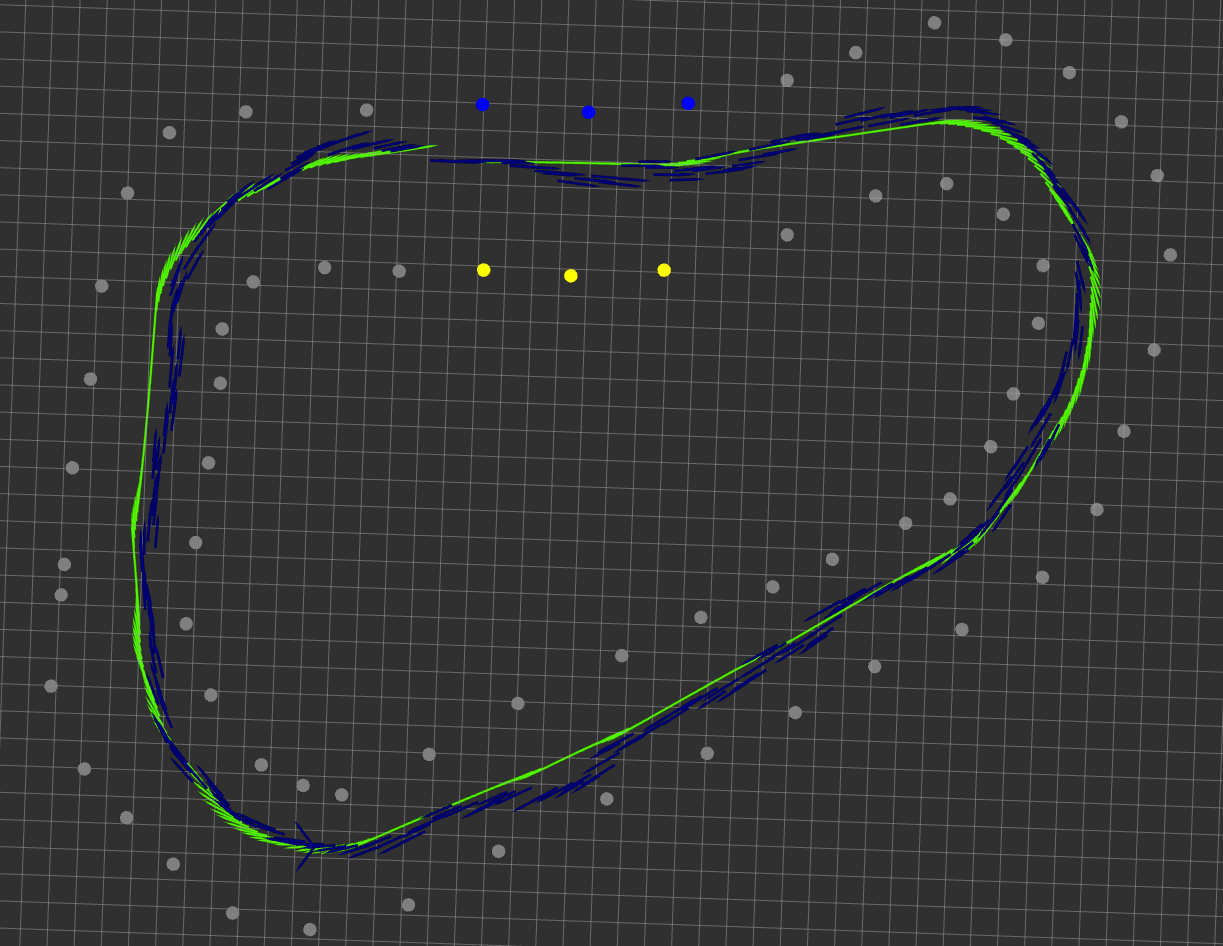
\includegraphics[width=\columnwidth]{images/gnss_pose.png}
	\caption{Fusing the GNSS position with $\sigma=7.5$}
	\label{fig:gnss_pose}
\end{figure}

\begin{table}[h]
	\begin{center}
		\begin{tabular}{|c|c|c|c|c|c|c|c|}
			\hline
			\multirow{2}{*}{\textbf{$\sigma$}} & \multicolumn{2}{c|}{\textbf{Final offsets}} &  \multicolumn{4}{c|}{\textbf{RMSE}} \\ \cline{2-7}
			  & $d$ & $\theta$ & $d$ & $\theta$ & $v$ & $\omega$ \\ \hline
			2.5 & 1.02 & 0.04 & 1.12 & 0.14 & 0.07 & 0.08 \\
			7.5 & 0.43 & 0.00 & 0.97 & 0.05 & 0.07 & 0.04 \\
			\hline
			
		\end{tabular}
		\caption{Final offsets and RMSE when fusing GNSS position}
	\end{center}	
\end{table}

\subsection{IMU + odometry + GNSS speeds}
It is interesting here not to fuse the GNSS position, to see clearly what happens without the shakes in the position. We can notice in figure \ref{fig:gnss_twist} that even if the error in position still accumulates a bit, the output is cleaner than only fusing IMU and odometry. Moreover, thanks to the track information, the error in orientation is bounded.

\begin{figure}[h]
	\centering
	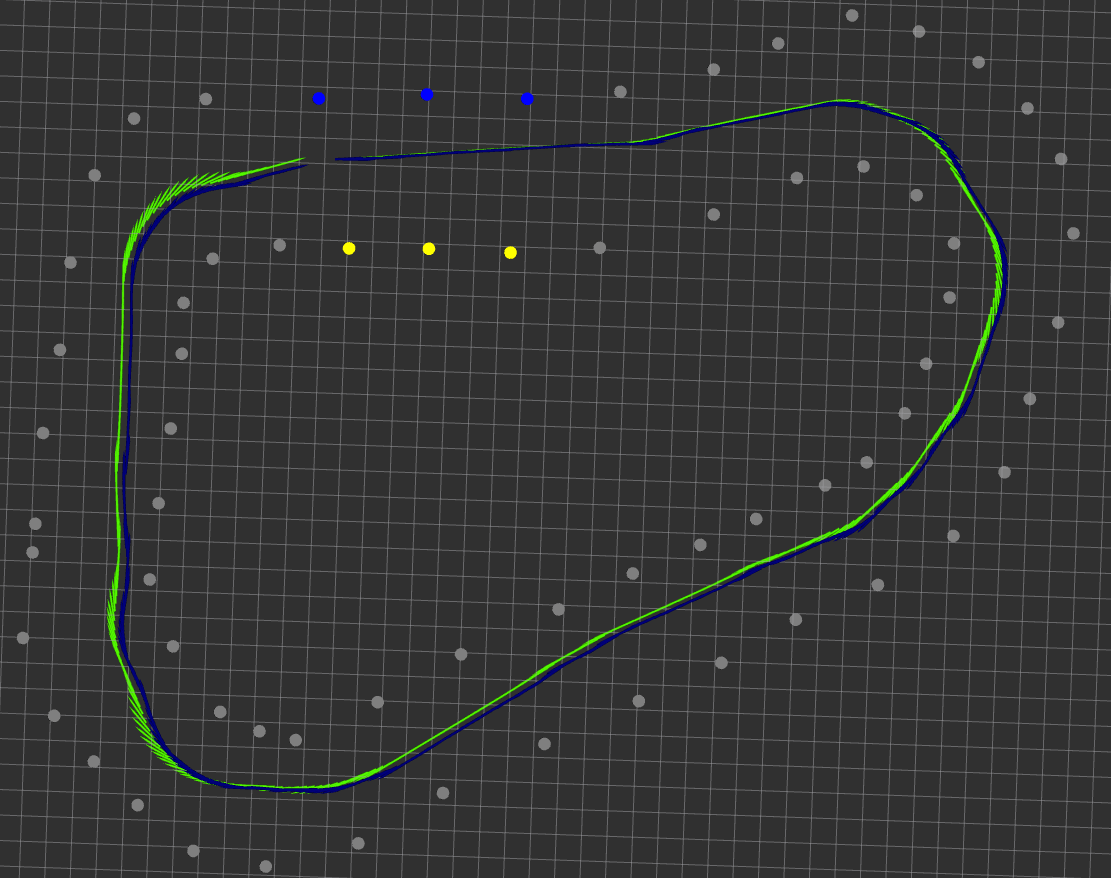
\includegraphics[width=\columnwidth]{images/gnss_twist.png}
	\caption{Fusing the GNSS speeds}
	\label{fig:gnss_twist}
\end{figure}

\begin{table}[h]
	\begin{center}
		\begin{tabular}{|c|c|c|c|c|c|c|}
			\hline
			\multicolumn{2}{|c|}{\textbf{Final offsets}} &  \multicolumn{4}{c|}{\textbf{RMSE}} \\ \hline
			$d$ & $\theta$ & $d$ & $\theta$ & $v$ & $\omega$ \\ \hline
			0.35 & 0.03 & 0.39 & 0.77 & 0.06 & 0.05 \\
			\hline
			
		\end{tabular}
		\caption{Final offsets and RMSE when fusing GNSS speeds}
	\end{center}	
\end{table}


\subsection{IMU + odometry + GNSS speeds + cones}
Since the standard deviation of the cones detection is of 3 cm, the accuracy of this measurement is of great value for the estimation of the position. In straight line, the output of the filter is very good. But in turns, the cones update is badly shifting the position, probably because of small orientation errors to which the cones measurement is very sensitive. A quick fix could be to do the update only if the angular speed is under some threshold.

In this configuration, since the data association is provided, the absolute localisation problem can be tackled: starting with a wrong initial state, the filter quickly converges towards the true state.

\begin{table}[h]
	\begin{center}
		\begin{tabular}{|c|c|c|c|c|c|c|}
			\hline
			\multicolumn{2}{|c|}{\textbf{Final offsets}} &  \multicolumn{4}{c|}{\textbf{RMSE}} \\ \hline
			$d$ & $\theta$ & $d$ & $\theta$ & $v$ & $\omega$ \\ \hline
			0.06 & 0.01 & 0.42 & 0.50 & 0.06 & * \\
			\hline
			
		\end{tabular}
		\caption{Final offsets and RMSE when fusing the cones (because of the orientation bug, the RMSE in $\omega$ is not relevant. The RMSE in $\theta$ is probably affected as well)}
	\end{center}	
\end{table}

\begin{figure}[h]
	\centering
	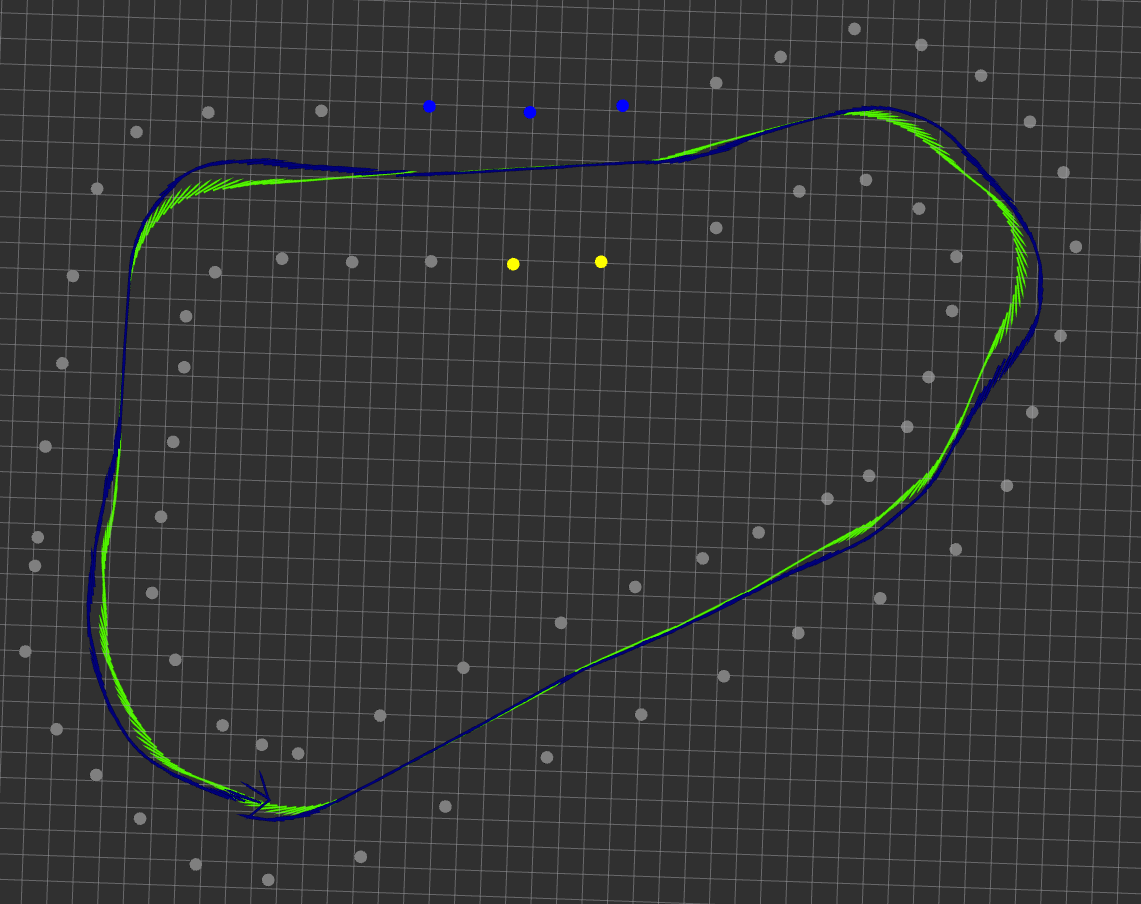
\includegraphics[width=\columnwidth]{images/cones.png}
	\caption{Fusing the cones position}
	\label{fig:cones}
\end{figure}


% SECTION: THE SOURCE CODE
\section{THE SOURCE CODE}
The source code can be found on GitHub at: \url{https://github.com/CorentinChauvin/ukf-localisation}. All the instructions to install and launch it can be found in the README file.

The interesting files to look at are:
\begin{itemize}
	\item the UKF implementation, in \textit{ukf\_localisation / src / ukf\_localisation.py}
	\item the cones detection faking, in \textit{gazebo\_simulation / eufs\_gazebo / nodes / cones\_perception.py}
	\item the odometry noising, in \textit{gazebo\_simulation / eufs\_gazebo / nodes / odometry\_publisher.py}
	\item a video of the running UKF, in \textit{REPORT / demo\_ukf\_localisation.mp4}
\end{itemize}


% SECTION: CONCLUSION
\section{CONCLUSION}
The presented Unscented Kalman Filter is able to fuse the various sensors mounted on the Formula Student car of KTH. The behaviour of its implementation has been studied in a realistic Gazebo simulation. It has been showed that even if the filter provides nice looking output, it is not perfect, and the accuracy of the state estimate wouldn't be enough in a driverless context. The main problem comes from the prediction phase using the IMU, which leads to very bad predictions. Some alternatives have been mentioned.

The next steps of this work could be to set up \texttt{robot\_localization} for the car. This ROS package contains a robust implementation of a UKF which could give a good comparison of what we could expect from a good filter. Then, one could use this knowledge to investigate weaknesses of the implementation and fix it (some fixes have been mentioned). Finally, it would be a nice ending to try the code on the real car. The code is already ready to work on the current system, and new interesting issues would probably surface.


% BIBLIOGRAPHY
\begin{thebibliography}{}
    \bibitem{ProbabilisticRobotics}
        Thrun, S., Burgard, W., and Fox, D. (2005). \textit{Probabilistic robotics}. MIT Press.
    \bibitem{RobustVehicleLocalization}
        Xiaoli Meng, Heng Wang, and Bingbing Liu. (2017). A Robust Vehicle Localization Approach Based on GNSS/IMU/DMI/LiDAR Sensor Fusion for Autonomous Vehicles.    
	\bibitem{GNSSVelocity}
	Salvatore Gaglione. (2015). How does a GNSS receiver estimate velocity?. \textit{InsideGNSS}.
	\bibitem{UKFForNonLinearEstimation}
	Eric A. Wan, and Rudolph van der Merwe. (2000). The Unscented Kalman Filter for Nonlinear Estimation.
	\bibitem{GeneralizedEKFImplementation}
	Thomas Moore, and Daniel Stouch. (2015). A Generalized Extended Kalman Filter Implementation for the Robot Operating System.
\end{thebibliography}

\end{document}